\thechapter{Description}
\thesection{Lighting}

\begin{figure}[h]
    \centering
        \begin{subfigure}[b]{0.2\textwidth}
        \includegraphics[width=\textwidth]{img/Lighting/ambient.png}
        \caption{Ambient}
        \label{fig:ambient}
    \end{subfigure}
    ~
    \centering
    \begin{subfigure}[b]{0.2\textwidth}
        \includegraphics[width=\textwidth]{img/Lighting/diffuse.png}
        \caption{Diffuse}
        \label{fig:diffuse}
    \end{subfigure}
     ~
    \centering
    \begin{subfigure}[b]{0.2\textwidth}
        \includegraphics[width=\textwidth]{img/Lighting/specular.png}
        \caption{Specular}
        \label{fig:specular}
    \end{subfigure}
    ~
    \centering
    \begin{subfigure}[b]{0.2\textwidth}
        \includegraphics[width=\textwidth]{img/Lighting/combined.png}
        \caption{All}
        \label{fig:combined}
    \end{subfigure}
    \caption{Phong Lighting}
    \label{fig:Lighting}
\end{figure}

The Phong lighting model is used, with specular, diffuse, and ambient light. Specular light concentrates light in one direction, providing highlights, diffuse light scatters light equally, providing shadows, and ambient light provides an equal amount of light to all parts of the surface from every direction. 

\begin{figure}[h]
    \centering
    \begin{subfigure}[b]{0.31\textwidth}
    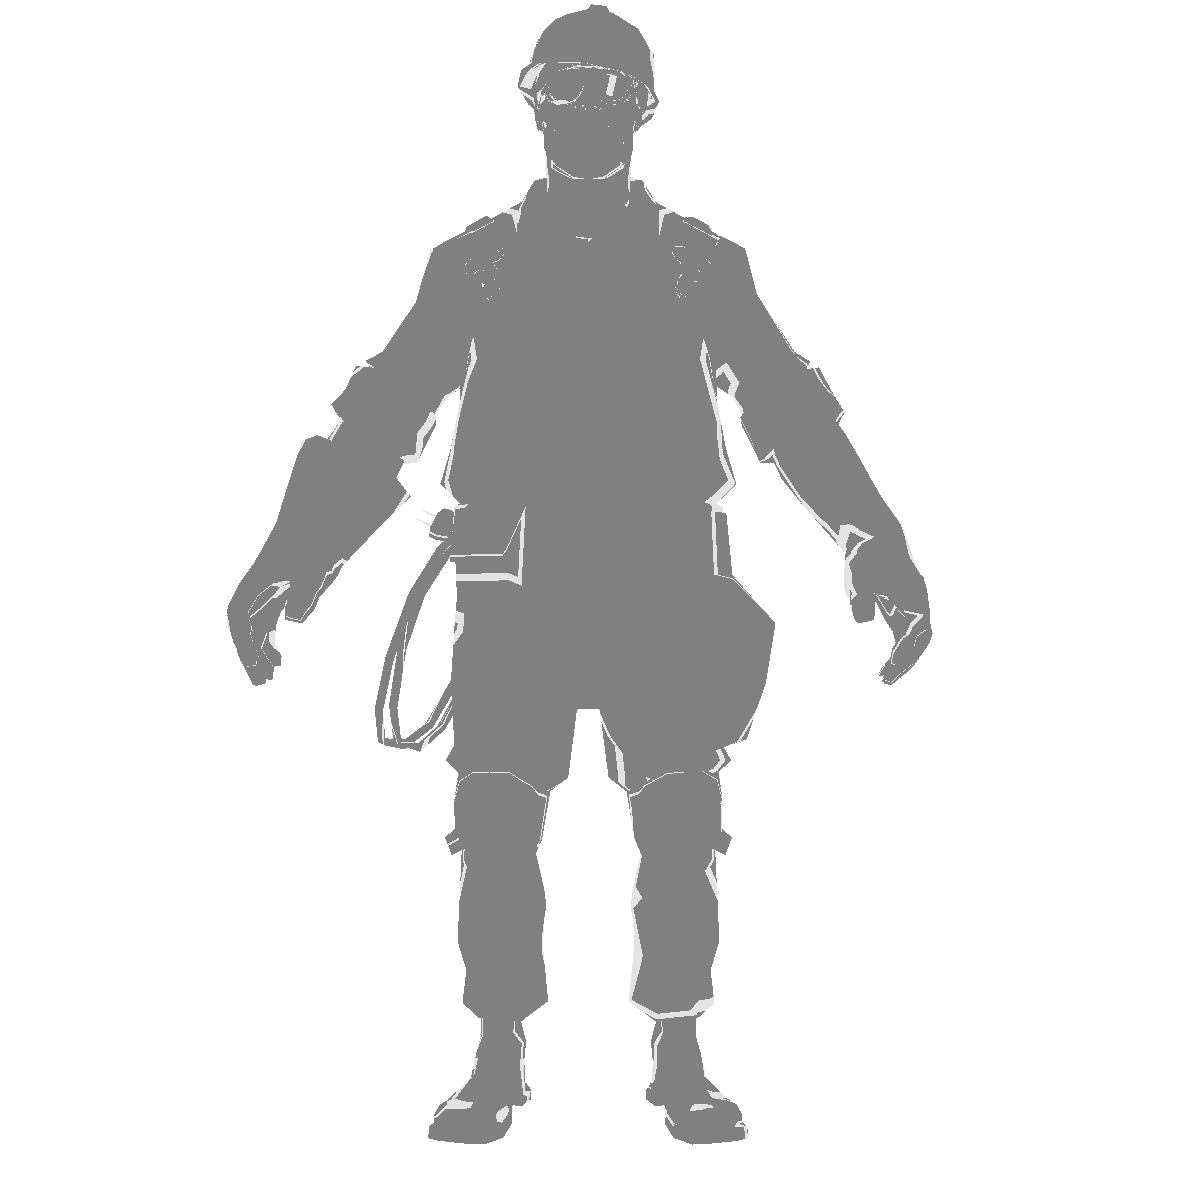
\includegraphics[width=\textwidth]{img/Lighting/Rim.png}
    \caption{Engineer}
    \label{fig:Rim}
    \end{subfigure}
    \centering
    \begin{subfigure}[b]{0.31\textwidth}
    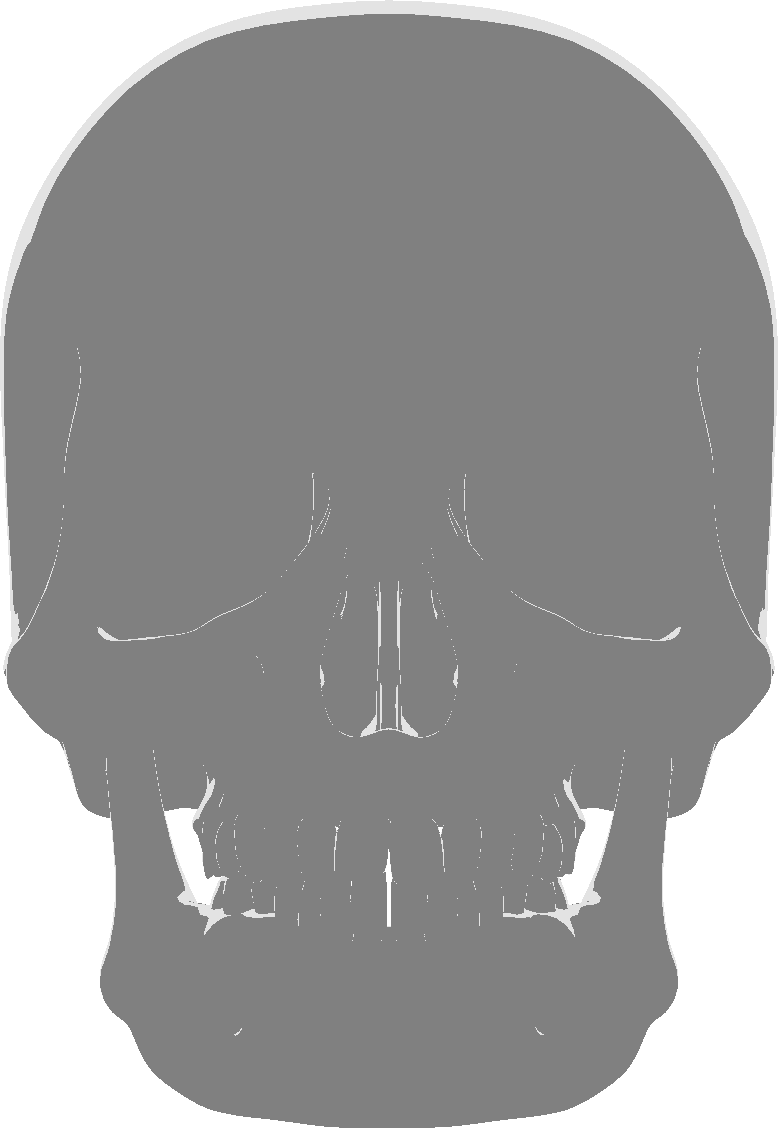
\includegraphics[width=\textwidth]{img/Lighting/RimSkull.png}
    \caption{Skull}
    \label{fig:RimSkull}
    \end{subfigure}
    \caption{Rim Lighting}
    \label{fig:RimLighting}
\end{figure}

Rim lighting is also added to provide additional highlights and increase the cartoon appearance of the render as specular highlights are not that effective. It highlights edges of the model perpendicular to the light within a range. This is likely as properties of the model's material is consistent throughout it's entire texture. It highlights the edge of the object, and as a result improves the rendering from some angles, but appears incorrect from some models that do not have smooth curves, and is highly dependant on the distance of the light from the object. 

\newpage 
\begin{lstlisting}[language=C]
vec4 ambient, diffuse, specular, rim, ltColor;
float d = dot(ptLightNorm, ptNorm);

// add phong lighting
ambientPortion = ambientColour;
diffusePortion = diffuseColour * d;
halfway = normalize(ptLightNorm - ptNorm);
s = max(dot(ptNorm, halfway), 0.0) ^ 2;
specularPortion = specularColour  * s;

// add rim lighting
float r = 1 - d;
if (r > 0.9 && r < 1.1)
    rimPortion = vec4(0.4, 0.4, 0.4, 1);

lighting = ambientPortion + diffusePortion
         + specularPortion + rimPortion;
\end{lstlisting}

Lighting is implemented in the fragment shader, rather than in the vertex shader, decreasing efficiency as it must be calculated for every fragment rather than the relatively small number of vertices, but providing more precise results. Our implementation of phong lighting is as described in \cite{texbook}, and the model can be displayed with either a directional or point light source.

% referring to the colour discretization process
\thesection{Cel shading}
Cel shading refers to an NPR technique where to better simulate a cartoon art style, the tones of 
an image are broken down into bands. The colour palette of a scene is reduced to a handful of colours.
The technique simulates how an artist might draw an image, where only a few shades are used, and few
separate colours are used.

To perform cel shading, a number of discrete bands n must be chosen. Higher values for n produce more 
bands of colour, which leads to less harsh contrast in the image, but fewer bands create more contrast,
and therefore a more dramatic effect. To get the final colour of a pixel, the RGB values are divided by
n+1, which returns the index of the band. Then, the index is multiplied by the size of the band, which
produces the final colour. Examples of cel shading for a particular model are shown in 
\autoref{fig:cel-band-comparison}. 

\begin{figure}[h]
    \centering
    \begin{subfigure}[b]{0.15\textwidth}
        
\includegraphics[width=\textwidth]{img/cel-shading-n1.png}
        \caption{n = 1}
        \label{fig:cel-shading-n1}
    \end{subfigure}
    ~
    \begin{subfigure}[b]{0.15\textwidth}
        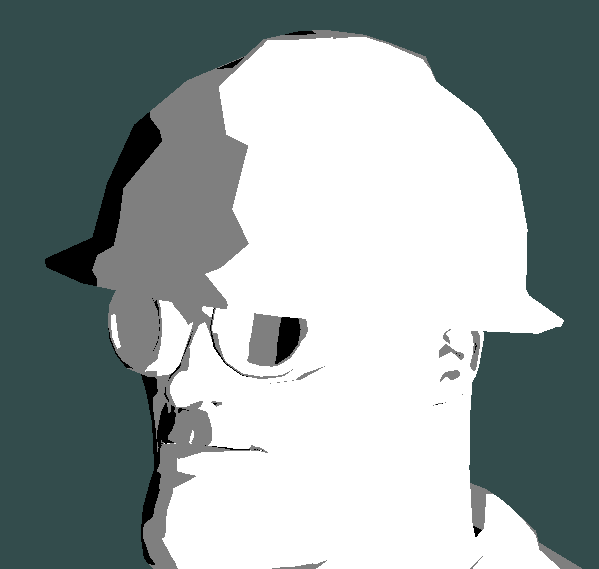
\includegraphics[width=\textwidth]{img/cel-shading-n2.png}
        \caption{n = 2}
        \label{fig:cel-shading-n2}
    \end{subfigure}
    ~
    \begin{subfigure}[b]{0.15\textwidth}
        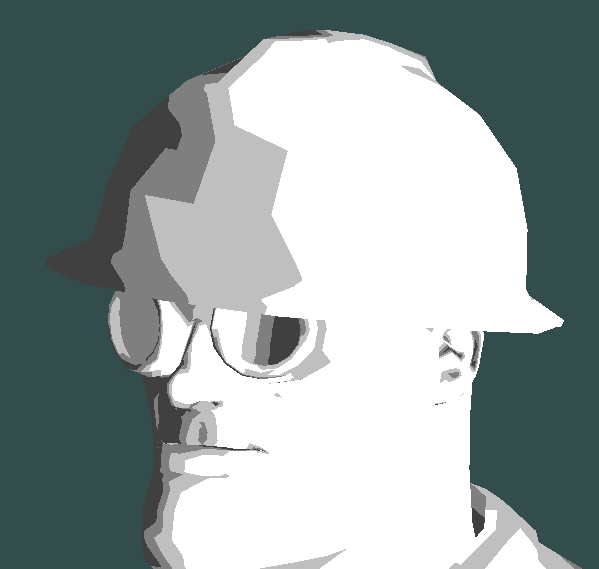
\includegraphics[width=\textwidth]{img/cel-shading-n4.png}
        \caption{n = 4}
        \label{fig:cel-shading-n4}
    \end{subfigure}

    \begin{subfigure}[b]{0.15\textwidth}
        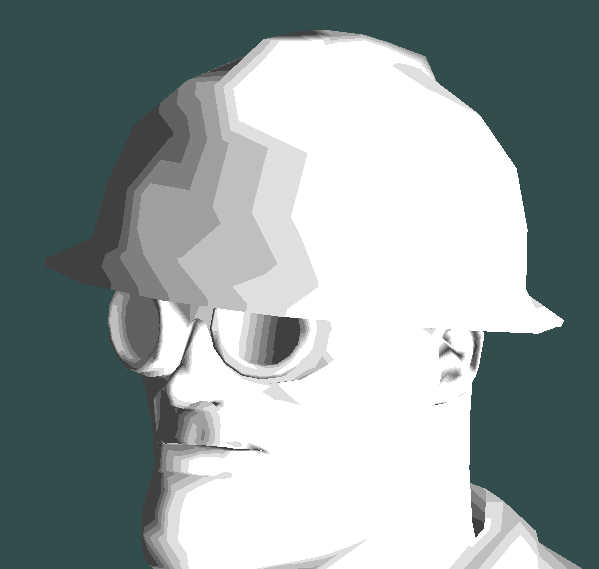
\includegraphics[width=\textwidth]{img/cel-shading-n8.png}
        \caption{n = 8}
        \label{fig:cel-shading-n8}
    \end{subfigure}
    ~
    \begin{subfigure}[b]{0.15\textwidth}
        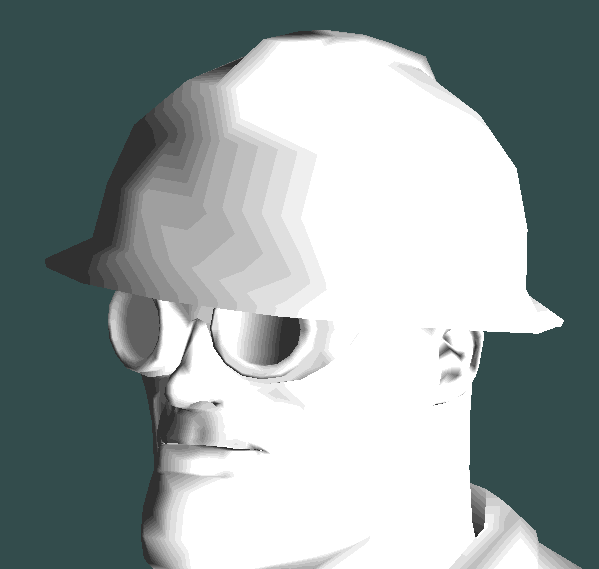
\includegraphics[width=\textwidth]{img/cel-shading-n16.png}
        \caption{n = 16}
        \label{fig:cel-shading-n16}
    \end{subfigure}
    ~
    \begin{subfigure}[b]{0.15\textwidth}
        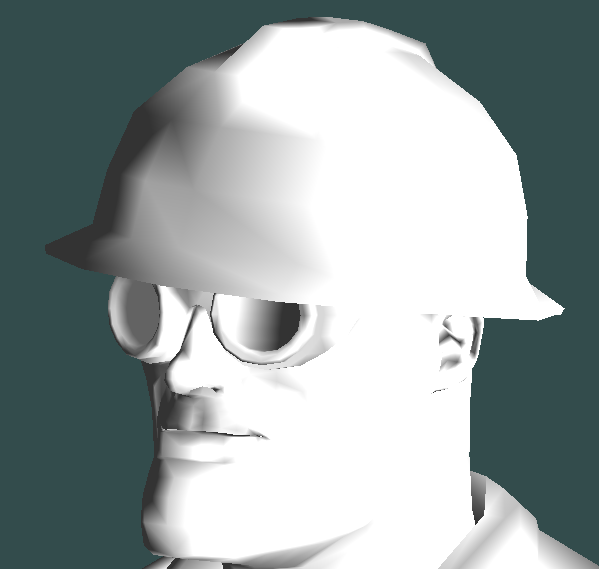
\includegraphics[width=\textwidth]{img/cel-shading-none.png}
        \caption{None}
        \label{fig:cel-shading-none}
    \end{subfigure}
    \caption{Comparison of number of cel shading bands}
    \label{fig:cel-band-comparison}
\end{figure}

One can notice sharp edges on the model. This is implementation specific, and happens because the 
colour passed to the fragment shader is interpolated between vertices by OpenGL. Normally, this creates 
a smooth effect and saves processing power, but when performing cel shading, it can destroy the effect, 
so it is turned off. Unfortunately, doing so creates jagged lines in models with a low polygon count, 
but the effect is  not as noticeable for higher polygon count models, such as in 
\autoref{fig:cel-shading-high-poly}. 

\begin{figure}[h]
    \centering
    \begin{subfigure}[b]{0.15\textwidth}
        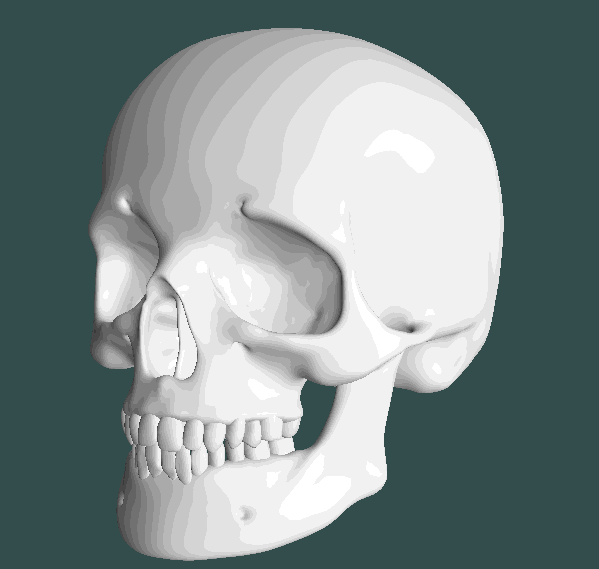
\includegraphics[width=\textwidth]{img/cel-shading-highpoly-n18.png}
        \caption{n = 18}
        \label{fig:cel-shading-high-poly-n18}
    \end{subfigure}
    ~
    \begin{subfigure}[b]{0.15\textwidth}
        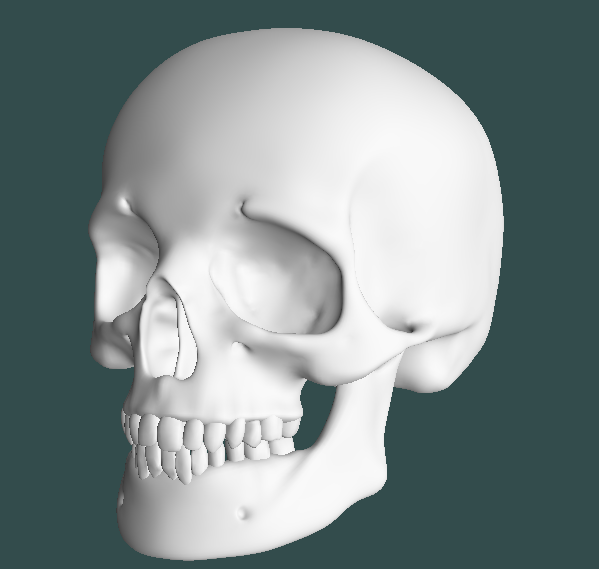
\includegraphics[width=\textwidth]{img/cel-shading-highpoly-none.png}
        \caption{None}
        \label{fig:cel-shading-high-poly-none}
    \end{subfigure}
    \caption{Cel shading with a high polygon count model}
    \label{fig:cel-shading-high-poly}
\end{figure}

% referring to the lines between the model and the background
\thesection{Outlines}
This is done by drawing lines on all the outer edges of the model. So as to clearly break it up form the background. As well as to give it a more stylized look. It is a commonly used technique in none photorealstic rendering. Even more so when trying to emulate a hand draw style.

\begin{figure}[h]
    \centering
    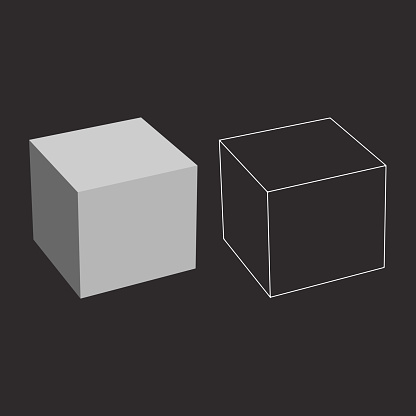
\includegraphics[width=0.5\textwidth]{img/Contour.jpg}
    \caption{An overview of stages in the rendering step}
    \label{fig-render-overview}
\end{figure}

% referring to the lines within the front facing side of the model that are added in
\thesection{Suggestive contours}
Suggestive Contours are a little more complex. Properly stated, “ Suggestive contours are lines drawn on clearly visible parts of the surface, where a true contour would first appear with a minimal change in viewpoint.”  \cite{Contours} Simplified, what this means is that suggestive contours are lines drawn on top of a model where the model is highly concave. So as the show deapth.

This helps to break up the form of the model in a way similar to how one dose when drawing with pencil and paper. This technique if most comonly used in situations where the model is atempting to look like a darwing or was made with a limited color palette.

\begin{figure}[h]
    \centering
    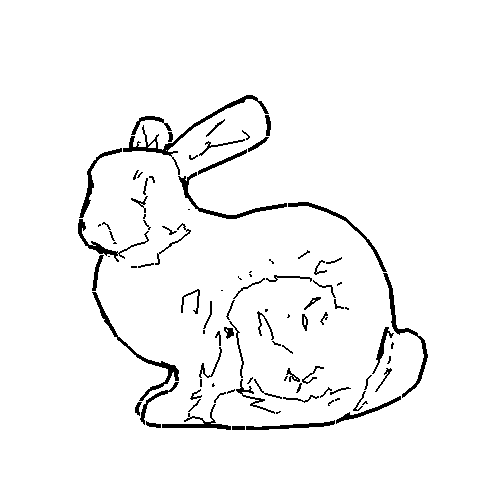
\includegraphics[width=0.5\textwidth]{img/SuggestiveContours.png}
    \caption{An overview of stages in the rendering step}
    \label{fig-render-overview}
\end{figure}

\newpage
\thesection{Textures}

\begin{figure}[h]
    \centering
        \begin{subfigure}[b]{0.2\textwidth}
        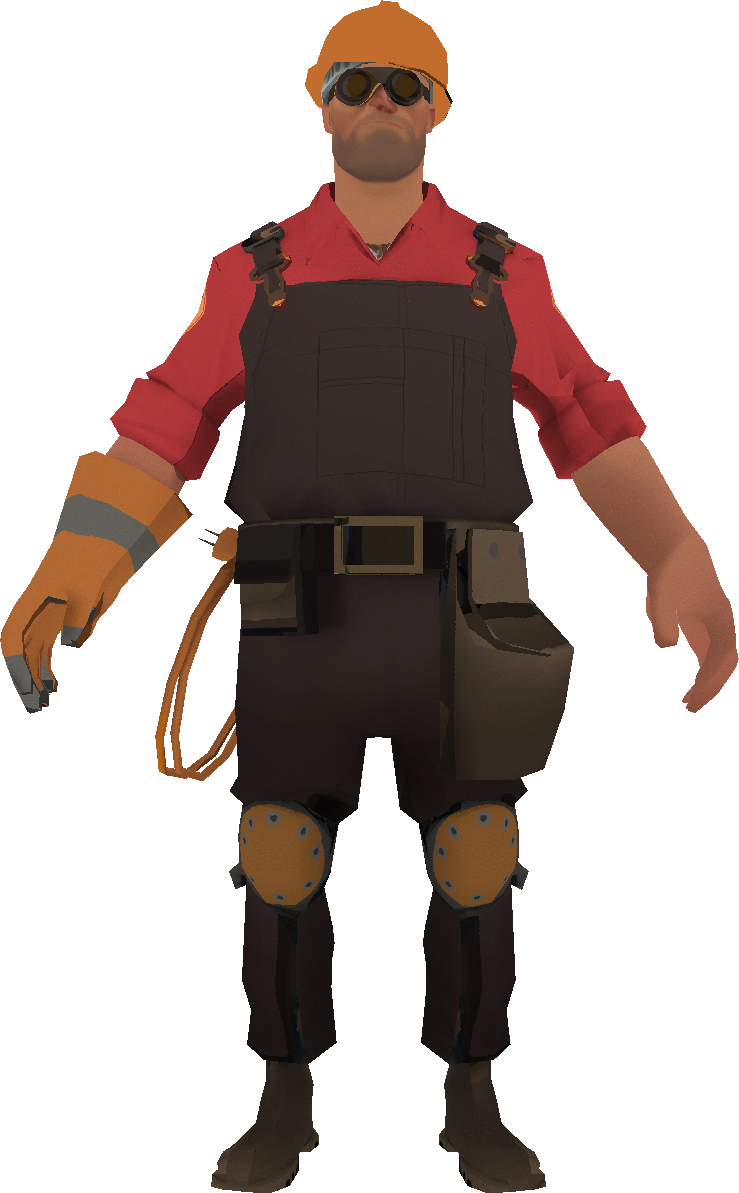
\includegraphics[width=\textwidth]{img/textures/Original.png}
        \caption{Original}
        \label{fig:Original}
    \end{subfigure}
    ~
    \centering
    \begin{subfigure}[b]{0.2\textwidth}
        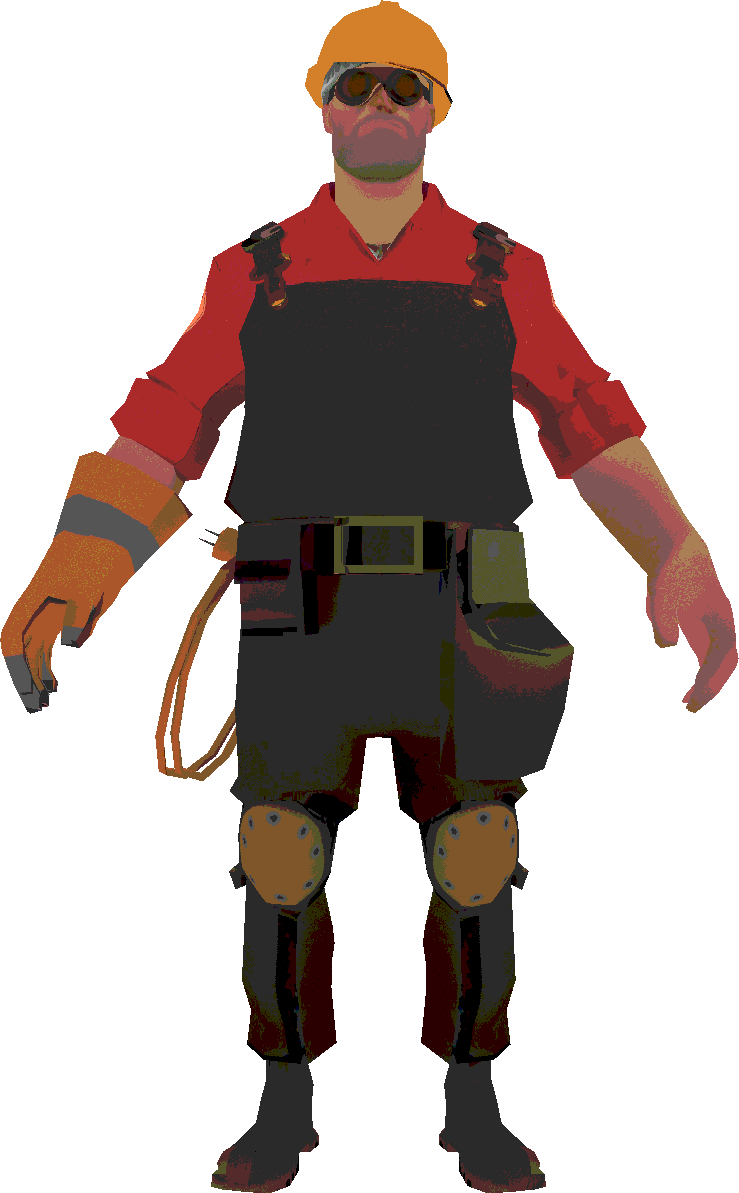
\includegraphics[width=\textwidth]{img/textures/CelShadeTexture6.png}
        \caption{6 Levels}
        \label{fig:CelShadeTexture4}
    \end{subfigure}
    ~
    \begin{subfigure}[b]{0.2\textwidth}
        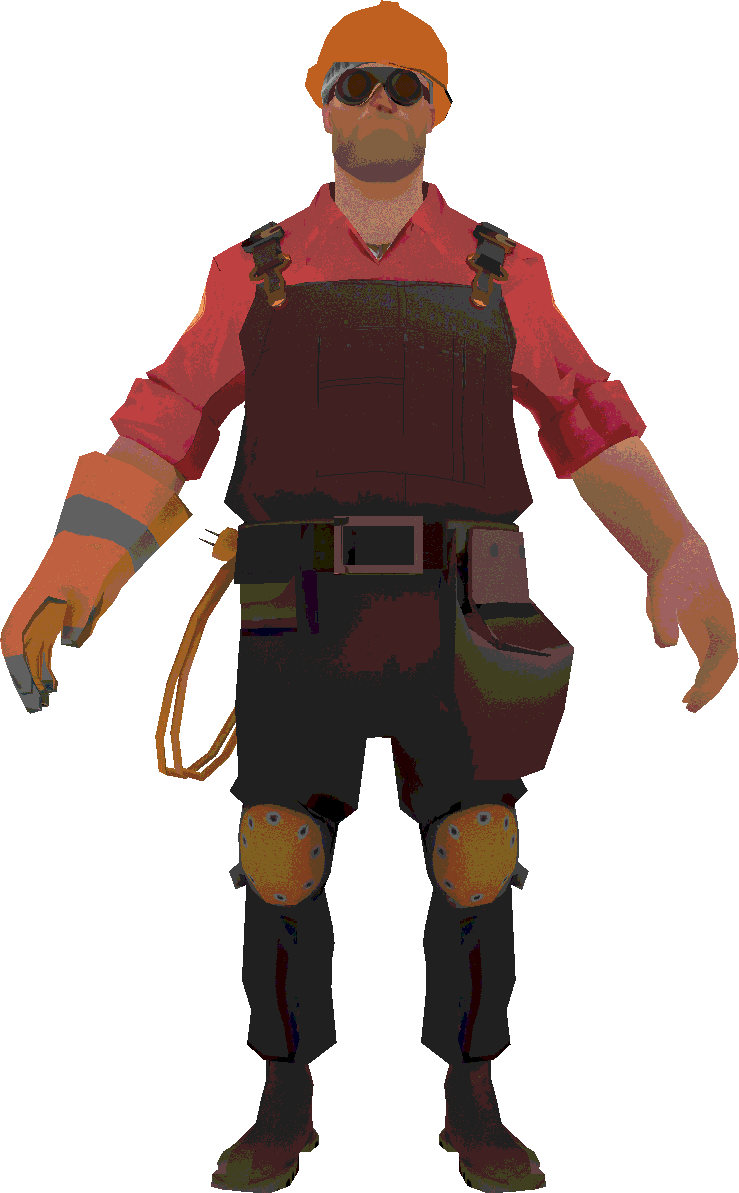
\includegraphics[width=\textwidth]{img/textures/CelShadeTexture8.png}
        \caption{8 Levels}
        \label{fig:CelShadeTexture8}
    \end{subfigure}
    %\begin{subfigure}[b]{0.2\textwidth}
     %   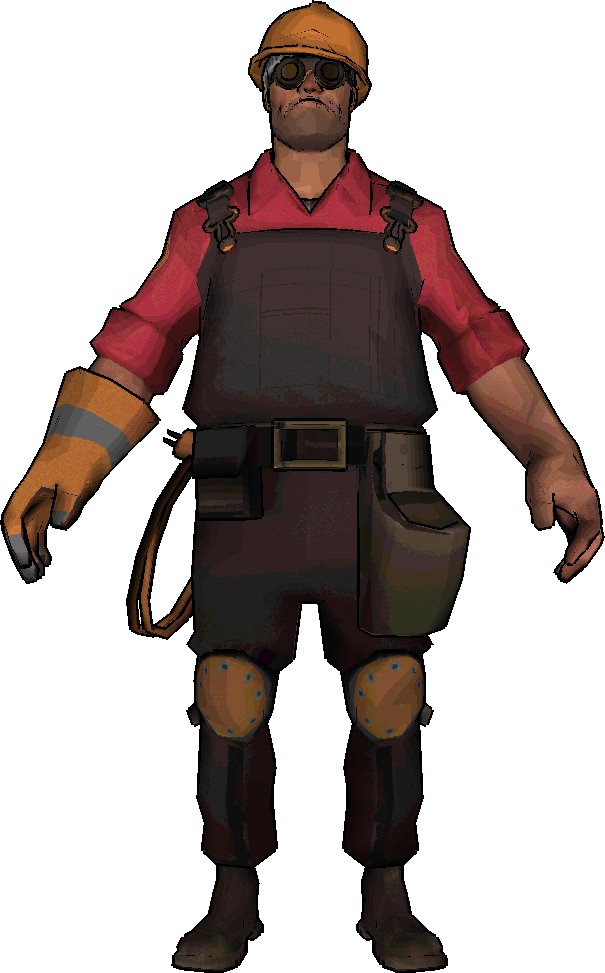
\includegraphics[width=\textwidth]{img/textures/TextureLightingCelShade.png}
    %    \caption{Final}
    %    \label{fig:TextureLightingCelShade}
    %\end{subfigure}
    \caption{Engineer}
    \label{fig:TexturesEngineer}
\end{figure}

%\begin{wrapfigure}{r}{0.4\textwidth}
\begin{figure}
\centering
\begin{subfigure}[b]{0.15\textwidth}
        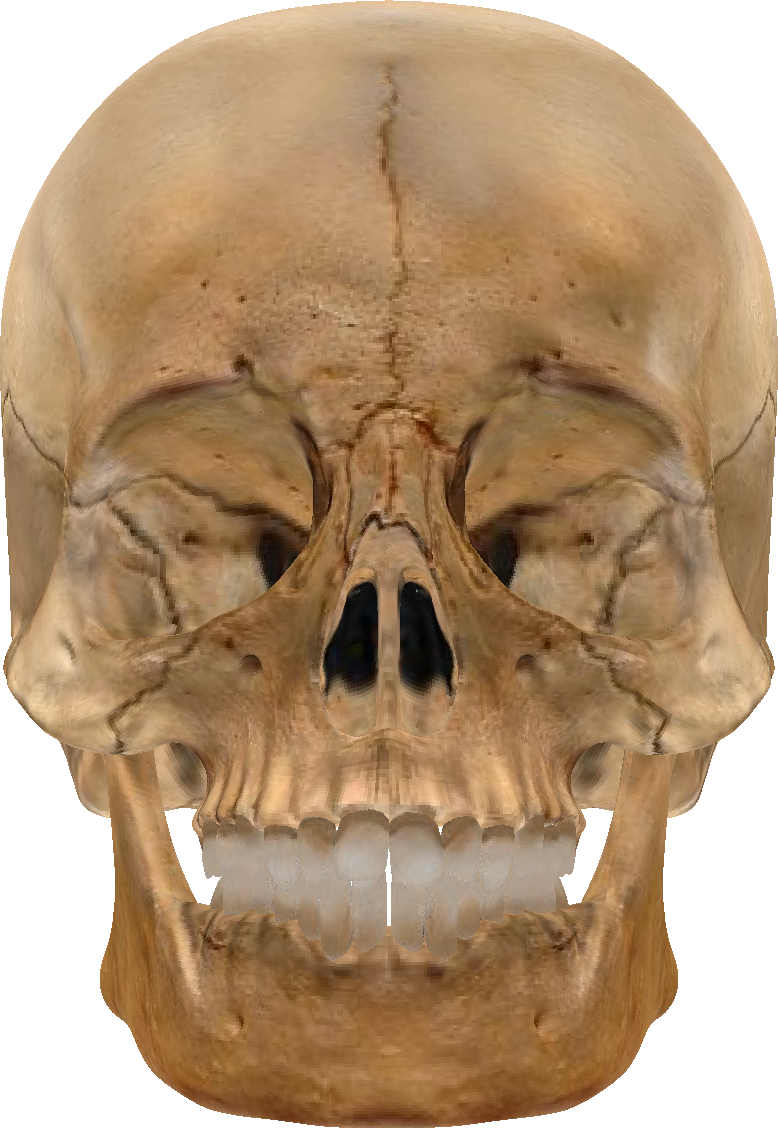
\includegraphics[width=\textwidth]{img/textures/OriginalSkull.png}
        \caption{Original}
        \label{fig:OriginalSkull}
\end{subfigure}
    ~
    \begin{subfigure}[b]{0.15\textwidth}
        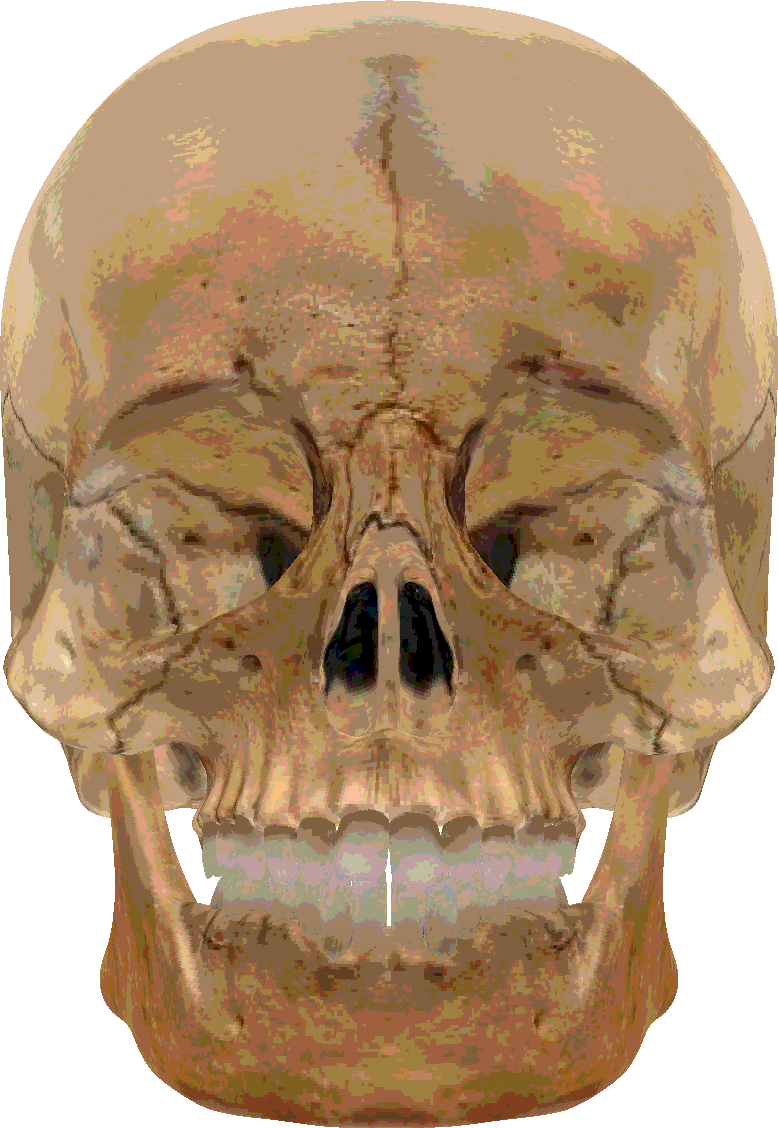
\includegraphics[width=\textwidth]{img/textures/CelShadeTexture8Skull.png}
        \caption{8 Levels}
        \label{fig:CelShadeTexture8Skull}
    \end{subfigure}
\caption{Skull}
\end{figure}
%\end{wrapfigure} 

Texture coordinates are loaded from the initial .obj file and stored with each vertex, and can then be used both to render the model with its original texture or to replace the texture with another image. In the fragment shader textures are used to map fragments to the color at the fragment's texture coordinate interpolated from the stored vertex coordinate. The color mapped by the coordinate in the model's textures can then be further modified through cel shading so photo realistic versions are rendered in a consistent toon style.

\begin{figure}[h]
    \centering
        \begin{subfigure}[b]{0.3\textwidth}
        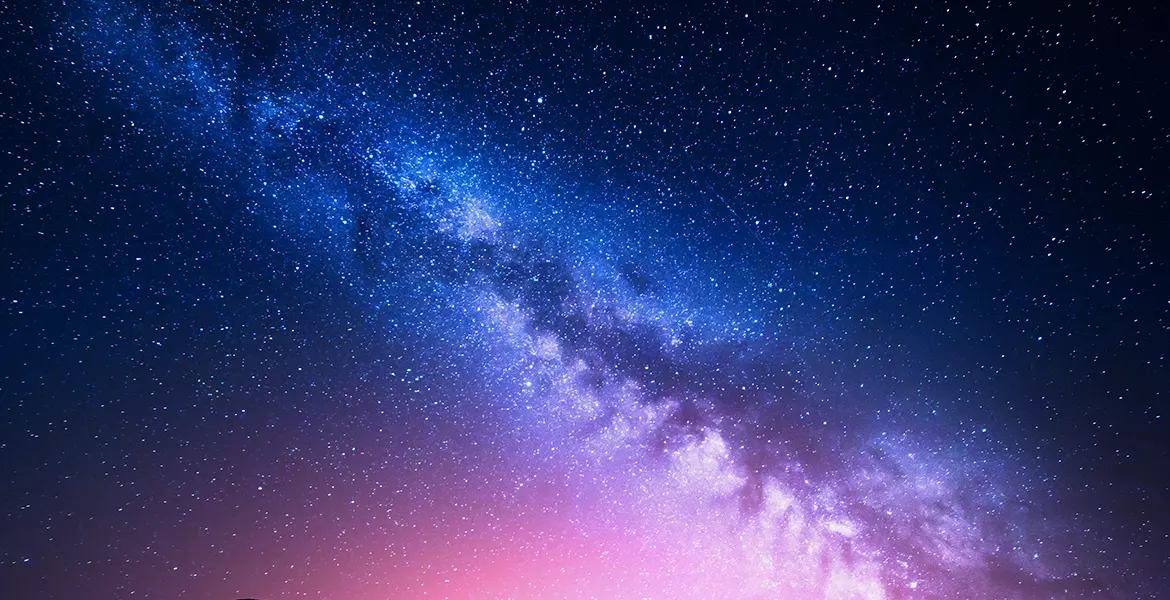
\includegraphics[width=\textwidth]{img/textures/space.png}
        \caption{Initial Texture}
        \label{fig:Space}
    \end{subfigure}
    ~
    \centering
    \begin{subfigure}[b]{0.25\textwidth}
        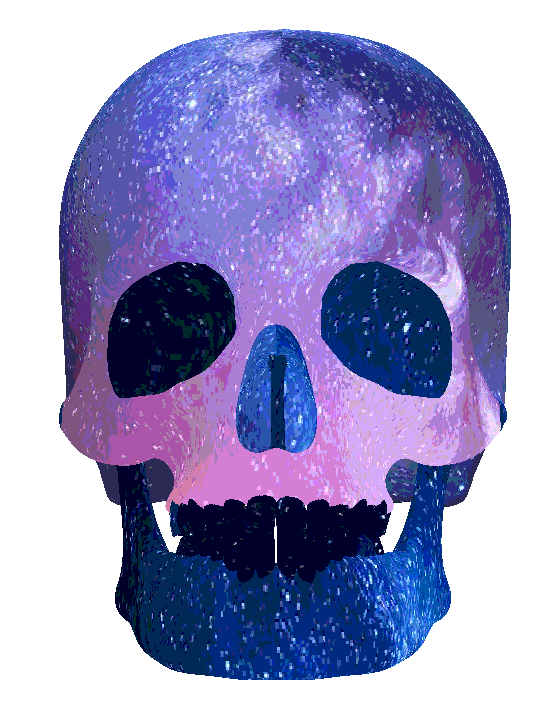
\includegraphics[width=\textwidth]{img/textures/TextureReplacementSkull.png}
        \caption{Skull}
        \label{fig:TextureReplacementSkull}
    \end{subfigure}
     ~
    \centering
    \begin{subfigure}[b]{0.2\textwidth}
        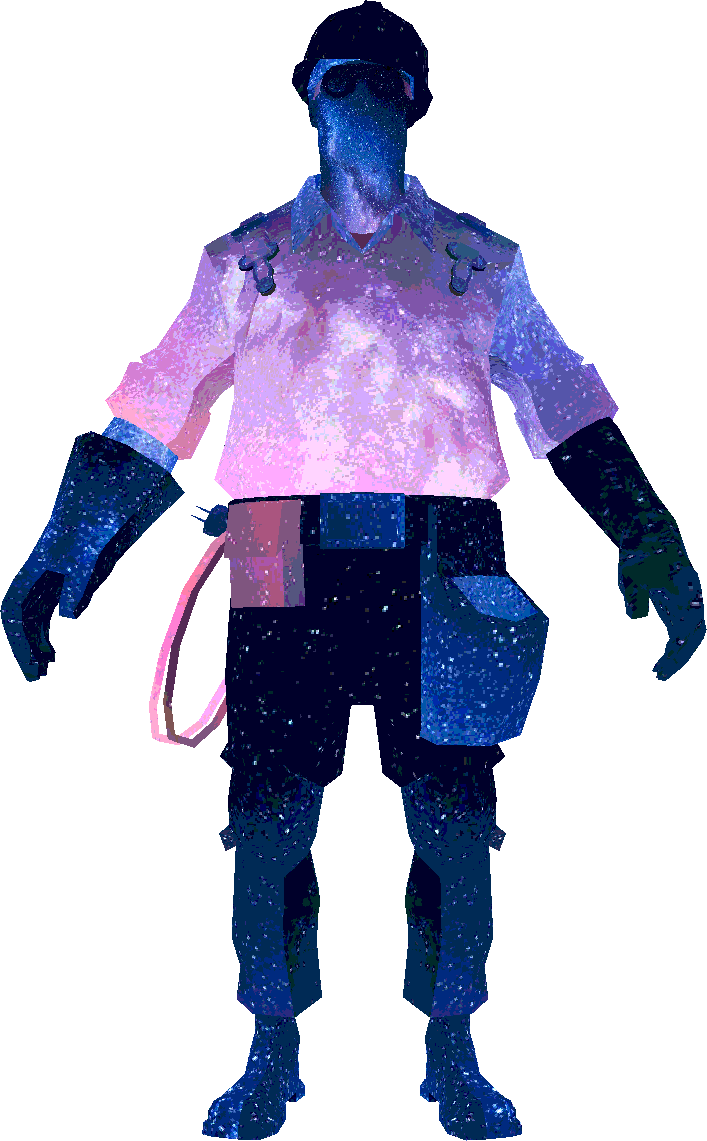
\includegraphics[width=\textwidth]{img/textures/TextureReplacement.png}
        \caption{Engineer}
        \label{fig:TextureReplacement}
    \end{subfigure}
    \caption{Replaced Textures}
    \label{fig:TexturesReplacement}
\end{figure}

Using a photo-realistic image transformed through cel shading as the new texture can produce interesting renders with the same process used for the original textures.


% probably could add a section about lighting the model
\thesection{System overview}
The described features were implemented into a real-time rendering system. The system itself 
was written in OpenGL3. Specifically, we used LWJGL's implementation of OpenGL. We took advantage
of the vertex and fragment shaders that OpenGL3 requires to be used. The use of vertex and fragment
shaders allows us to implement most algorithms on the GPU, which saves CPU cycles and increases the
performance of the application.

Essentially, our system is a real-time renderer for 3D models that handles lighting, arbitrary
textures, and allows shading effects to be toggled on or off for comparison. A camera is supported
so that the model can be examined from a variety of viewing angles. A high-level overview of the
system is presented in \autoref{fig-sys-overview}.

% I'm going to include a flow chart or something here to have a visual aid
\begin{figure}[h]
    \centering
    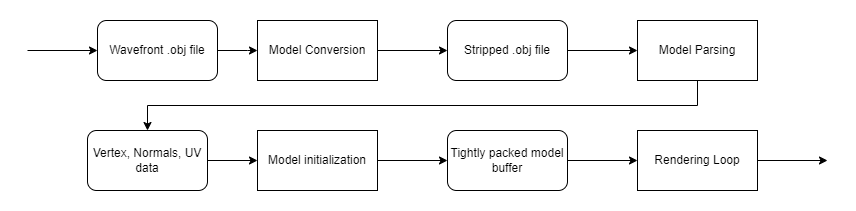
\includegraphics[width=0.5\textwidth]{img/system-overview.png}
    \caption{An overview of stages in the system}
    \label{fig-sys-overview}
\end{figure}

% model_converter | Conversion stage
The first stage of our system takes in .obj files and reformats parts of the file in order to make
it easier to parse. This was implemented as a separate Python program, since it needs only be done 
once per model.
% WavefrontParser, MtlParser | Parsing stage
The second stage of the system parses a .obj file to produce a prototype of a Model that our system
is later able to render. In doing so, the vertices, vertex normals, and texture coordinates from the
file are packed into the prototype model. Additionally, the indices that use this data to define
faces of the model are also read. At this stage, textures are also read in for the model from the
.mtl file referenced by the  .obj file. One caveat is that imported models should be triangulated,
as our system has no procedure in place to triangulate polygons.
% Model, setupBuffers | Initialization
The next stage of the system packs the Model data into a format that the vertex shader can 
understand. An strided array of nine floating point values per vertex is created. The first three
values each stride represent the vertex data, the next three are the vertex normal, and the final 
three contain texture coordinates. These values are passed as attributes to the vertex shader.
The buffer only ever has to be calculated once per model, so this stage does not repeat. 
% Model, .vs, .fs | Rendering
Every frame, each model is rendered. The render proceeds by passing light and camera parameters to 
the vertex shader, along with the vertex, vertex normal and texture coordinates from the previous 
stage. Two rendering stages happen for our program, the outline render loop, and the model render
loop. These stages are shown visually in \autoref{fig-render-overview}.

\begin{figure}[h]
    \centering
    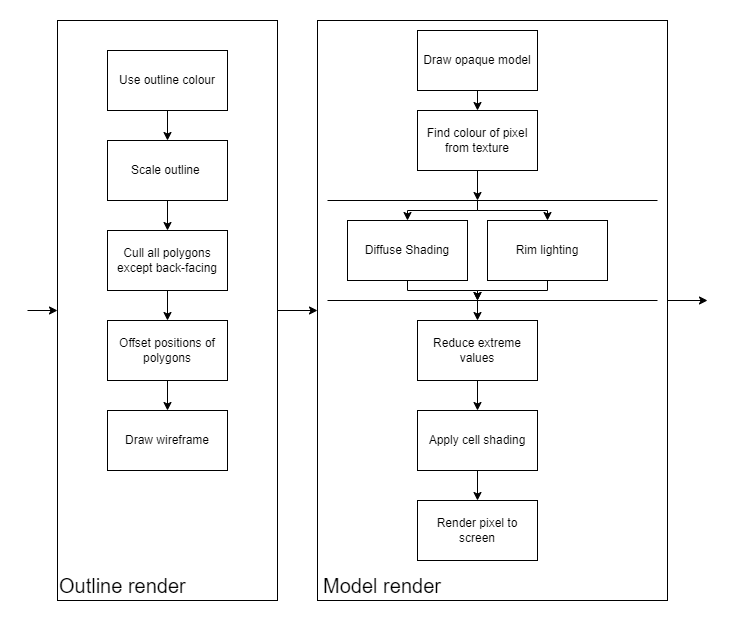
\includegraphics[width=0.5\textwidth]{img/rendering-overview.png}
    \caption{An overview of stages in the rendering step}
    \label{fig-render-overview}
\end{figure}

The outline render loop draws only the back faces of the model in a black wireframe. Edges
are drawn at a size of 5 pixels instead of the default 1 pixel, so they stick out from the model.
Furthermore, the polygons of the model are draw slightly offset to further accentuate the outlines.
One issue with this approach to drawing outlines is that the size of the outlines is constant no 
matter the distance to the model, so far away objects end up with much more noticeable outlines
than closer models.

% a figure of the wireframe would be cool here

The model render loop handles the lighting and the cel shading of the object, and the its work is
done in the vertex and frament shaders. The steps are detailed below.

The vertex shader is the entry point for the OpenGL pipeline, so its main role is to forward the 
parameters that the fragment shader uses, and to specify the position of each vertex sent to it. 
Additionally, the vertex shader calculates the lighting normal.

The fragment shader does the bulk of the work of our application. In the fragment shader, two main
procedures happen. First, the colour of the lighting for the fragment is found. This is a multi-step
process that involves applying diffuse lighting, rim lighting, and reducing extreme light and dark 
values in order to preserve the colour of the model. Afterward, cel shading is applied to discretize
the colours of the model. 

% a figure of the model without the wireframe seems appropriate here

% a figure of the model with wireframe seems appropriate here
% maybe all three images could be in a single figure

\autoref{fig:teapot-comparison} shows the rendering process at three stages, drawing the outline,
drawing the inner model, and the combined final result. One drawback to this approach of drawing
outlines is that the rendering pipeline is used twice per model. However, it may be not quite as 
intensive since only back faces are drawn, and the wireframe of the model is not filled.



\begin{figure}[h]
    \centering
    \begin{subfigure}[b]{0.2\textwidth}
        
\includegraphics[width=\textwidth]{img/teapot-wireframe.png}
        \caption{Outline}
        \label{fig:outline-render}
    \end{subfigure}
    ~
    \begin{subfigure}[b]{0.2\textwidth}
        
\includegraphics[width=\textwidth]{img/teapot-outline-noshade.png}
        \caption{Unshaded}
        \label{fig:model-noshade}
    \end{subfigure}
    ~
    \begin{subfigure}[b]{0.2\textwidth}
        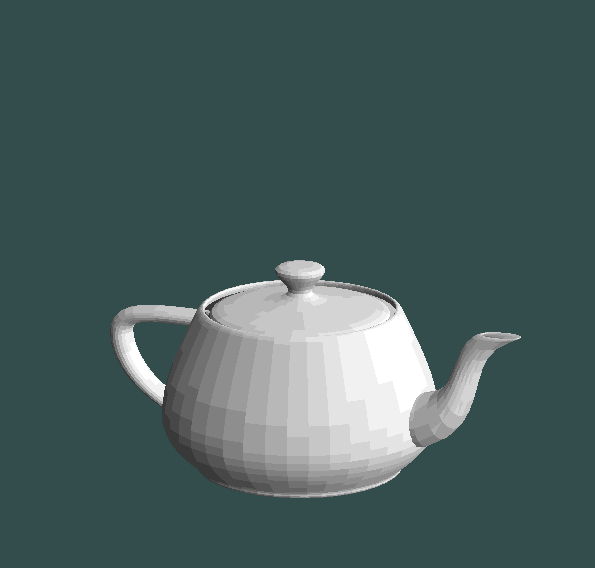
\includegraphics[width=\textwidth]{img/teapot-model.png}
        \caption{Shading}
        \label{fig:model-render}
    \end{subfigure}
    ~
    \begin{subfigure}[b]{0.2\textwidth}
        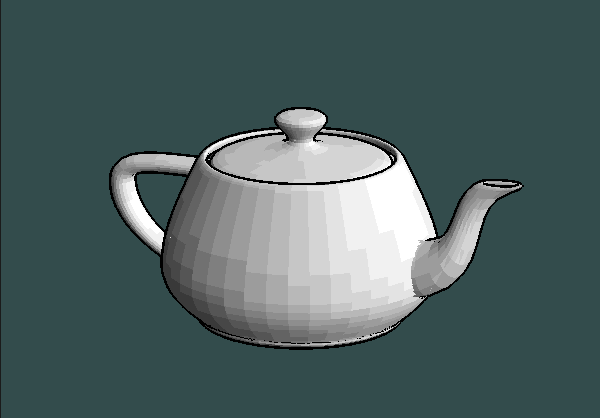
\includegraphics[width=\textwidth]{img/teapot-complete.png}
        \caption{Final}
        \label{fig:complete-render}
    \end{subfigure}
    \caption{Comparison of output at each rendering stage}
    \label{fig:teapot-comparison}
\end{figure}


